% This is LLNCS.DEM the demonstration file of
% the LaTeX macro package from Springer-Verlag
% for Lecture Notes in Computer Science,
% version 2.4 for LaTeX2e as of 16. April 2010
%
\documentclass{llncs}
%
\usepackage{makeidx, graphicx, subfigure}  % allows for indexgeneration
\usepackage{float,rotating,subfigure}
%
\begin{document}
%
\frontmatter          % for the preliminaries
%
\pagestyle{headings}  % switches on printing of running heads
\addtocmark{Hamiltonian Mechanics} % additional mark in the TOC

\mainmatter              % start of the contributions
%
\title{Zoomable Video Playback on Mobile Devices by Selective Decoding}
%
\titlerunning{Selective Decoding}  % abbreviated title (for running head)
%                                     also used for the TOC unless
%                                     \toctitle is used
%
\author{Feipeng Liu \and Wei Tsang Ooi}
%
\authorrunning{Wei Tsang Ooi \and Feipeng Liu} % abbreviated author list (for running head)
%
%%%% list of authors for the TOC (use if author list has to be modified)
\tocauthor{Wei Tsang Ooi and Feipeng Liu}
%
\institute{Department of Computer Science,\\National University of Singapore,\\13 Computing Drive Singapore 117417,\\
\email{\{liuf0005, ooiwt\}@comp.nus.edu.sg}}

\maketitle              % typeset the title of the contribution

\begin{abstract}
Many mobile devices are not capable of playing high definition video smoothly. Moreover video playback on mobile devices drains the battery quickly. We propose a method named selective decoding to increase video playback frame rate and reduce power consumption. 
Selective decoding is based on the idea that users are usually interested in only part of a video scene. It will be more efficient if only the user's Region of Interest (ROI) is decoded. To enable selective decoding, we analyzed various dependency relationships among macroblocks in MPEG4 Part 2 Simple Profile codec, traced the macroblocks that are needed to decode the ROI, and modified standard decoding process to decode macroblocks selectively based on the trace. Our experiments on Android platform show that selective decoding can improve playback frame rate by up to 193.3\% and reduce energy consumption by up to 64.5\%.
\keywords{selective decoding, zoomable video, energy saving, Region of Interest playback}
\end{abstract}

%
\section{Introduction}
Video playback is supported in most of today's typical mobile devices. A recent study shows 20\% people watch videos on their mobile devices\cite{webbusinessinsider}.

Despite its popularity, several issues of mobile video playback remain unaddressed. Firstly, because its heavy processing requirement, High Definition (HD) video playback is not supported on many mobile devices. Secondly, video playback is energy demanding, and the fast pace discharge of battery makes the mobile devices ununsable quickly. 

The screen on mobile devices is usually not large, despite its high resolution. Pinch zoom and pan gestures have been widely adopted to help users to view photos, maps and web pages. Recent research indicates zoom and pan are helpful for users when watching videos\cite{Khiem:2011:TUU:2072298.2071917}. However, the examination of existing mobile video players on iPhone and Android platforms tell us many of them do not support zoom and pan. And for those supporting these gestures, they simply scale the video up.

When a video is scaled up, only part of the video scene are displayed. The visible part is referred as Region-of-Interest (ROI). The simple scale and display approach for video playback is inefficient since the entire video scene is decoded but only part of it is displayed. This observation presents an opportunity to achieve more efficient video playback on mobile devices. 

We propose a software approach named selective decoding that improves the efficiency of zoomable video playback. As its name suggests, this approach decodes video selectively based on the ROI captured from user interactions. With the improved efficiency, it is hoped this approach can help to address the two issues mentioned previously.

Our work is based on MPEG4 Part 2 Simple Profile (SP) codec, however this approach should be applicable for other Discrete Cosine Transform (DCT) based video codec. We focus our work on the decoder side of the codec in the local playback context, but the principles and techniques could be extended to encoder and video playback in network streaming context. A typical MPEG4 SP decoder is illustrated as below,
\begin{figure}
\centering
%\vspace{2.5cm}
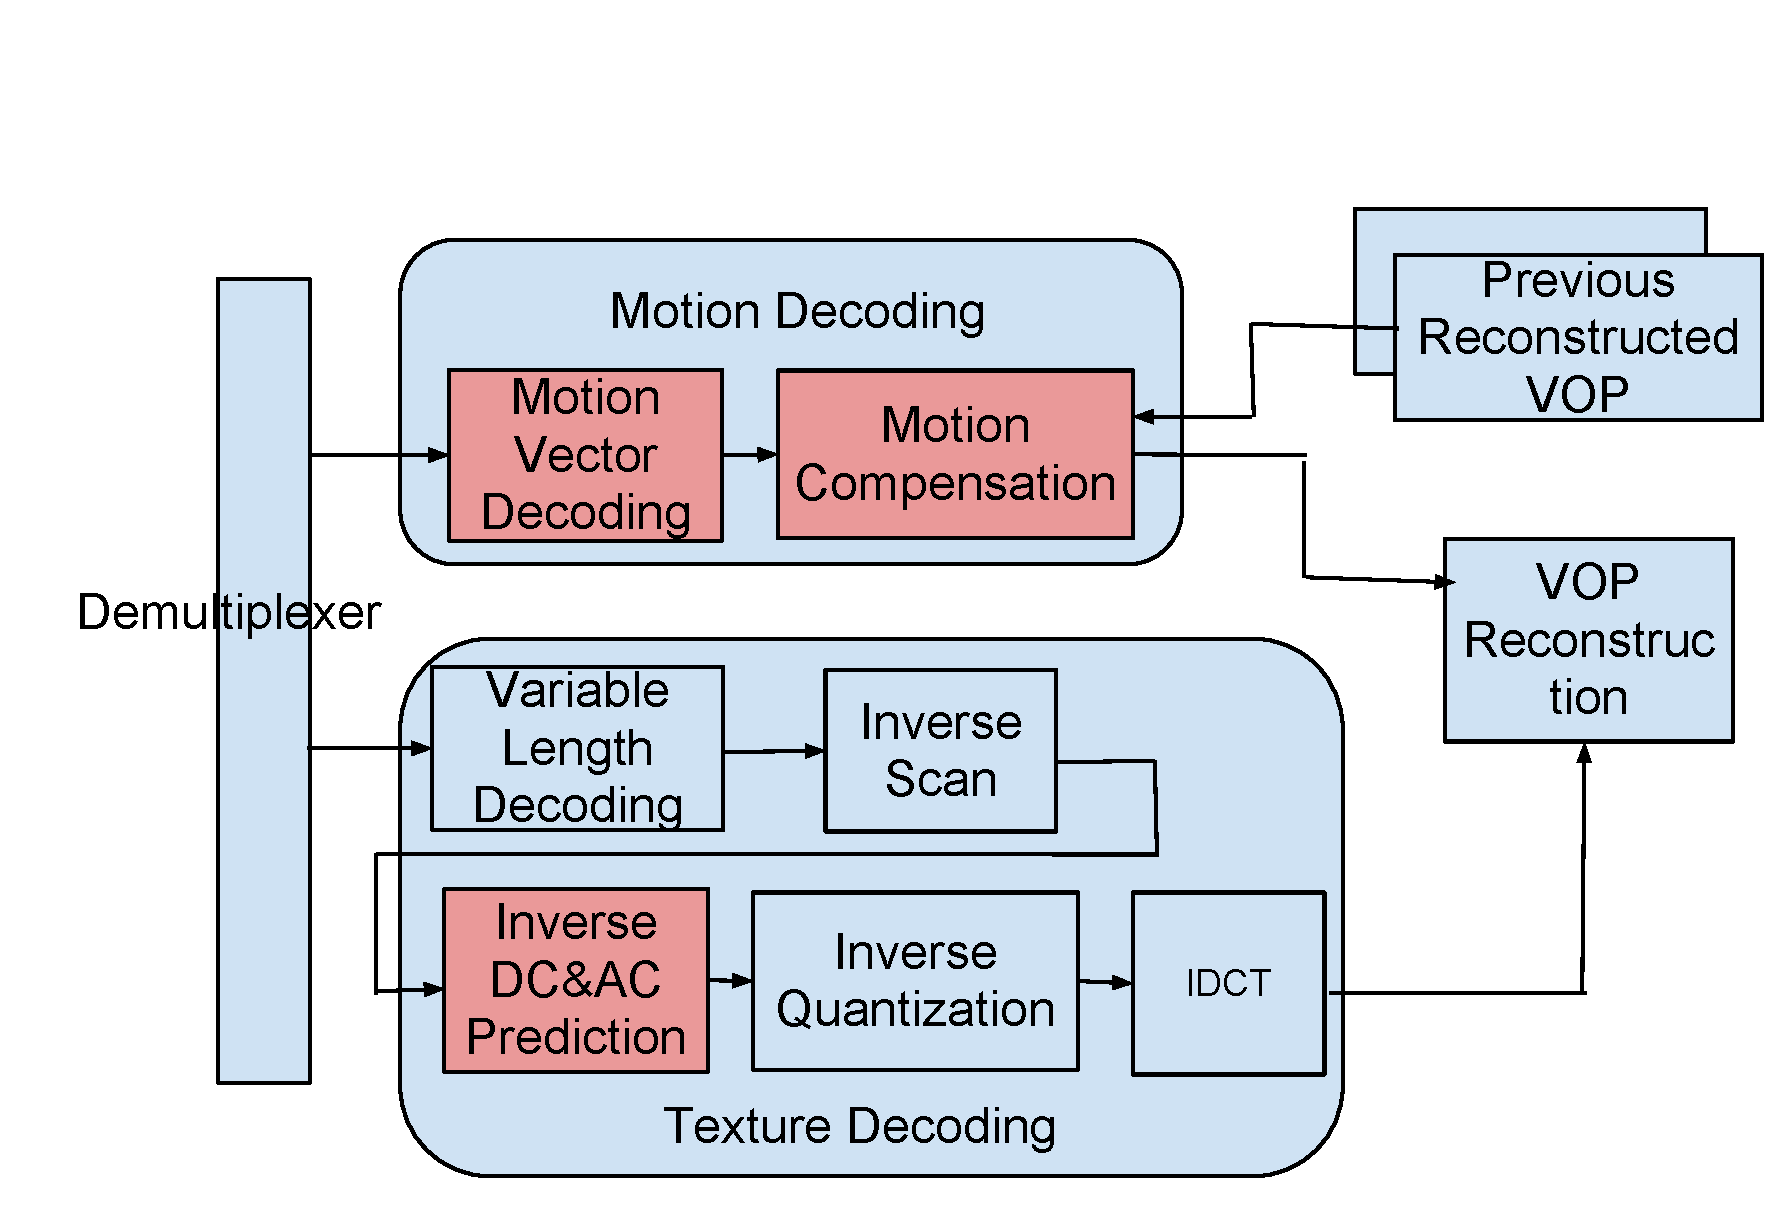
\includegraphics[height=4.5cm]{decoderb.eps}
\caption{A Typical MPEG4 Part 2 Decoder}
\end{figure}
The encoded bitstream is demultiplexed. The coded texture goes through the texture decoding and coded motion is processed by motion decoding. The decoder finally reconstructs the Video Object Plane (VOP). Note that the figure only depicts the core idea of MPEG4 SP decoder, lots of complexities are not covered. 

Various dependencies exist among macroblocks of a MPEG4 SP coded video. From the decoder's pespective, Inverse DC\&AC Prediction phase at Texture Decoding, and Motion Vector (MV) Decoding and Motion Compensation at Motion Decoding of a macroblock are carried out with reference to other macroblocks. Specifically, Inverse DC\&AC Prediction and Motion Vector Decoding are done with reference to other macroblocks in the current VOP, while motion compensation requires macroblocks from previous reconstructed VOP. Because of these dependencies, decoding the MBs of a ROI will require macroblocks outside of ROI to be decoded. 

The selective decoding approach preprocesses the video to obtain the dependencies and save them into files. At decoding, it computes a bitmask based on the dependencies for every VOP on the fly, where the selected macroblocks are marked as '1' and others are marked as '0'. The modified decoder then decodes the selected macroblocks accordingly to the bitmask. In this manner, the macroblocks that are necessary and sufficient to present a clear scene at ROI are decoded. 

In the rest of this paper, section 2 reviews related works. section 3 analyzes the dependencies in detail and discusses the offline computation of selective decoding. Online computation is covered in section 4, including the bitmask generation and modified decoder. Section 5 briefly describes different approaches that validates selective decoding. The proposed approach is implemented in Android platform and described in section 6. We evaluate selective decoding for both video playback frame rate and energy consumption in section 7 and finally conclude at section 8. 





  


  

\section{Related Work}
H.264/MPEG4 Advanced Video Coding (AVC) standard includes an extension supporting Scalable Video Coding (SVC)\cite{Schwarz07overviewof}. It enables transmission and decoding of partial bit streams to provide video of lower resolution and/or lower frame rate. SVC requires changes to both encoder and decoder and is not widely adopted yet. 

Supporting zoomable video through encoders has been explored by several research groups. Mavlankar etc. studied the optimal slice size for zoomable video in a network streaming context\cite{Mavlankar07optimalslice}. Feng etc. presented how to produce a video stream  with ROI cropping support by constraining the video compression process\cite{Feng:2011:SRC:2000486.2000491}. 

More works exist on zoomable video in network context, each with its own focus. Utilizing zoomable video to save bandwidth by refining the encoding process is studied\cite{Ngo:2011:AEZ:1943552.1943581}; Zoomable video on peer-to-peer streaming is explored\cite{Mavlankar_peer-to-peermulticast}; ROI prediction and tracking for streaming zoomable video is examined\cite{roi_pred}\cite{roi02}\cite{Fan03lookinginto}; multiple ROIs support is investigated\cite{multiroi}. 

In summary, extensive research has been done to enable zoomable video in network streaming context, with focus on video encoding process. To the best of our knowledge, no material has been found on enabling zoomable video from decoder in local playback context through the decoding process.  

\section{Offline Computation}
The offline computation of selective decoding retrieves the dependencies by partially decoding a video. It is essential to understand various dependencies in order to comprehend offline computation. For all subsequent discussions in this paper, we assume the video is in YCbCr420 color space, which means a macroblock contains four luminance blocks and two chrominance blocks.  
\subsection{Dependencies}
Two categories of dependencies can be identified, namely intra-frame dependency and inter-frame dependency. Dependencies are the reason why some macroblocks outside of ROI need to be decoded. By saving certain information, we can reduce the dependencies and improve the efficiency of selective decoding. Below we analyze the dependencies and introduce the methods to reduce them. 
\subsubsection{Intra-frame Dependency}
Intra-frame dependency refers to the dependencies among macroblocks within a single frame. There are two sources of intra-frame dependency, including DC\&AC Prediction and MV coding. 

DC\&AC Prediction is performed for I-macroblock when the header field short\_video\_header is set to '0'. It consists of two steps, namely reference block selection and prediction decoding. The reference block selection step can be illustrated by Fig 2.

\begin{figure}
\centering 
%\vspace{2.5cm}
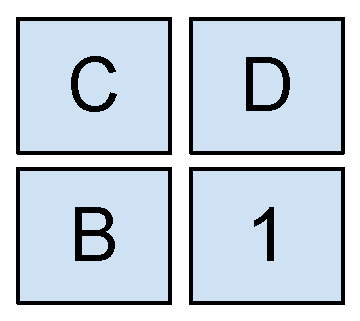
\includegraphics[height=1.2cm]{pred.eps}
\caption{DC\&AC Prediction Reference Block Selection}
\end{figure}
There are two candidate reference blocks for each block, the immediate left block and the immediate upper block. In addition, the upper left block is also needed in order to determine the reference block. To determine the reference block for block 1 in Fig 2, the following rule is applied,
%\begin{verbatim} 
{\tt \\if (|F(B)[0][0] - F(C)[0][0]| < |F(C)[0][0] - F(D)[0][0]|)\\
\indent predict from block D \\
else  \\
\indent predict from block B \\} 
%\end{verbatim}
F(B)[0][0], F(C)[0][0] and F(D)[0][0] refer to inverse quantized DC value of block B, C and D respectively. The selection rule indicates one block is dependent on three neighboring blocks. In the actual prediction decoding, the decoding block depends only on the selected reference block.

Two out of three blocks are only needed to determine the prediction direction, which is either up or left. A single bit is enough to record this information, with '0' indicating up and '1' referring to left. This reduces the dependency for a block from three to one.

MV of P-frame is differentially coded, which is the other source of intra-frame dependency. At motion decoding, the decoder recovers the MV values based on the decoded base values and residue values obtained from neighboring macroblocks. In selective decoding, the MVs are recorded to trace the Inter-frame Dependency, which is discussed next. Therefore the MVs can be read directly by decoder and no MV prediction decoding is needed. Thus the dependency due to MV prediction decoding is eliminated completely.
  
\subsubsection{Inter-frame Dependency}
Inter-frame dependency refers to the dependencies among macroblocks at different frames, which is caused by motion compensation coding. In MPEG4 SP, motion compensation decoding only occurs at P-macroblock of P-frame. The inter-frame dependency is illustrated as Fig 3.

\begin{figure}
\centering
%\vspace{2.5cm}
%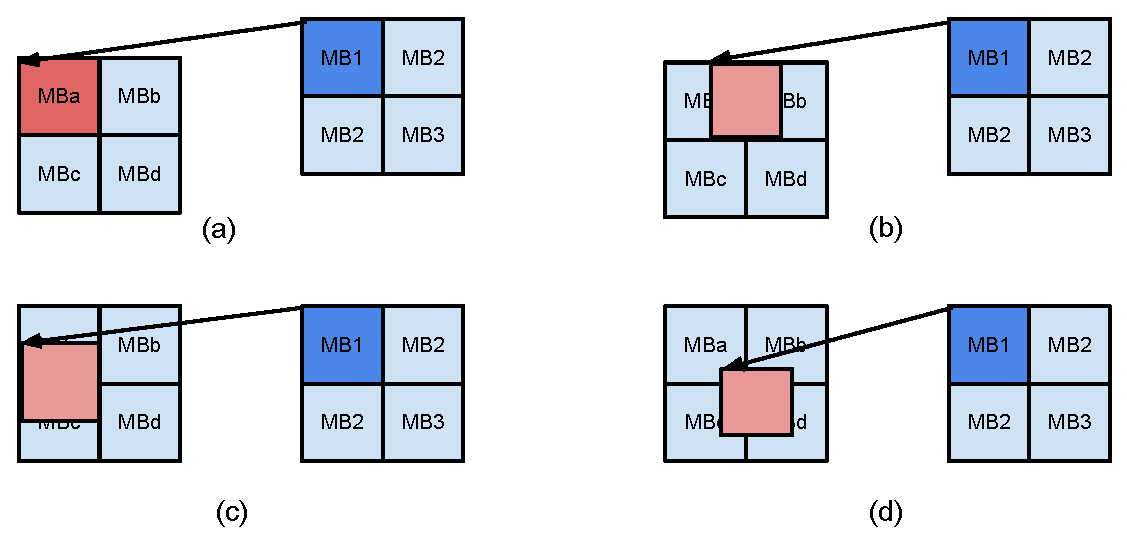
\includegraphics[height=2.5cm]{mm1.eps}
\subfigure[]{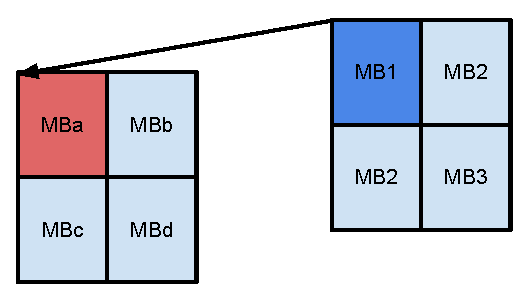
\includegraphics[height=1.15cm]{me1.eps}}
\quad
\subfigure[]{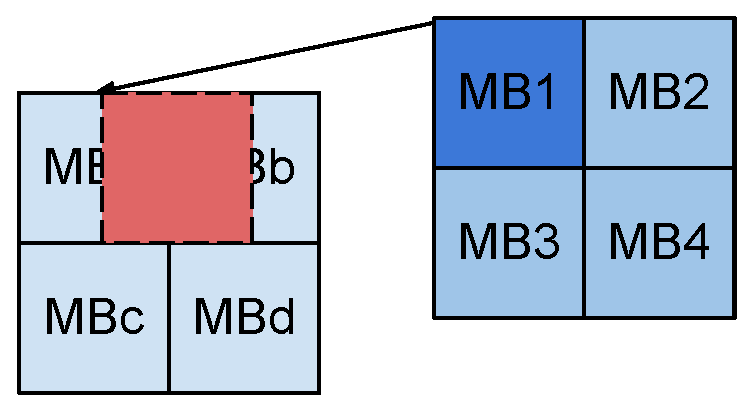
\includegraphics[height=1.15cm]{me2.eps}}
\quad
\subfigure[]{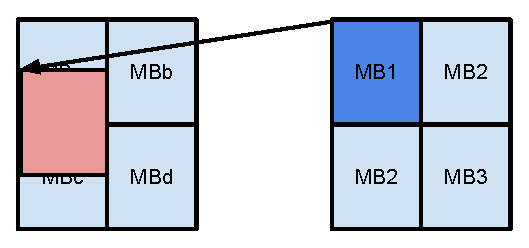
\includegraphics[height=1.15cm]{me3.eps}}
\quad
\subfigure[]{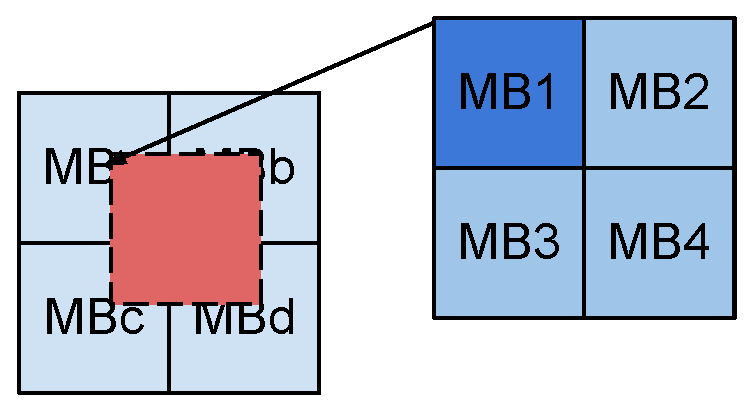
\includegraphics[height=1.15cm]{me4.eps}}
\caption{Different Cases of Motion Compensation Decoding}
\end{figure}
Motion compensation decoding is performed on MB1 of the current frame, with reference to a region of a previous frame. The number of dependent macroblocks depends on whether the reference region aligns with the macroblock boundary. As shown in Fig 3, MB 1 depends on one macroblock at (a), two macroblocks at (b) and (c), and four macroblocks at (d). 

Khiem etc. proposed an approach to reduce dependency due to motion compensation\cite{Ngo:2011:AEZ:1943552.1943581}. We adopted their technique in this research. Using the case in Fig 3(d) as an example, the approach is illustrated Fig 4.

\begin{figure}
\centering
%\vspace{2.5cm}
%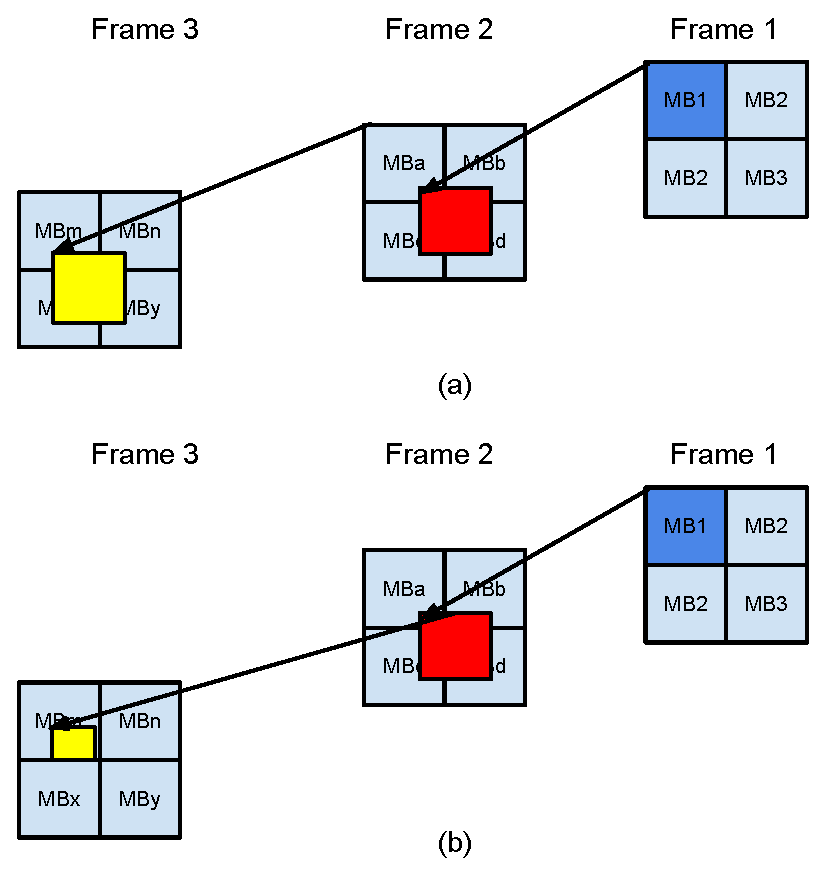
\includegraphics[height=2.5cm]{mm2.eps}
\subfigure[]{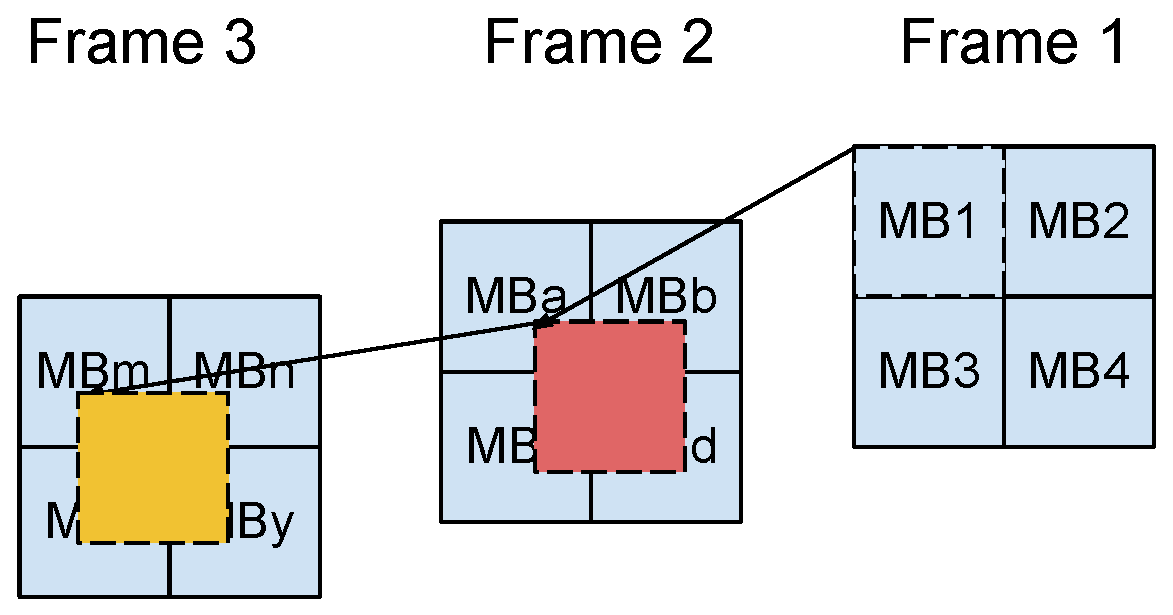
\includegraphics[height=2.0cm]{meo1.eps}}
\quad\quad
\subfigure[]{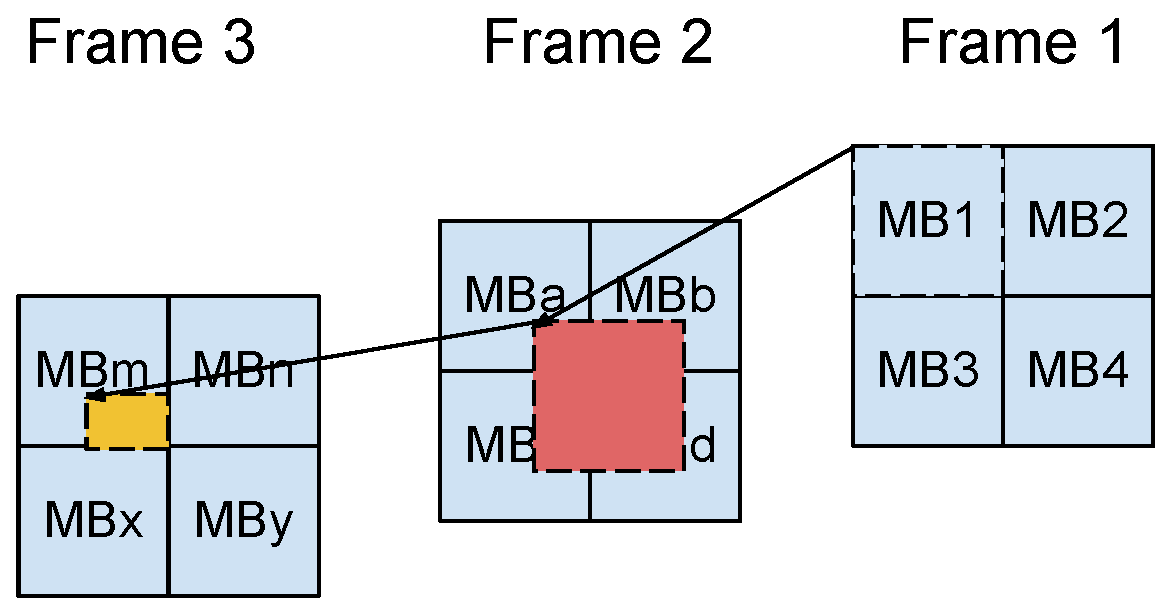
\includegraphics[height=2.0cm]{meo2.eps}}
\caption{Dependency Analysis for Motion Compensation}
\end{figure}

MB1 at Frame 1 depends on four macroblocks at Frame 2. MBa at Frame 2 depends on another four macroblocks at Frame 3. Dependency can be reduced by tracing it at pixel level. The dependency between Frame 1 and Frame 2 remains the same. But we do not really need all pixels at Frame 2 MBa. The region needed at MBa depends on only part of MBm at Frame 3. Therefore, the dependency for MBa between Frame 2 and 3 are reduced from four to one in this example.

\subsection{Dependency Files}
The offline computation partially decodes a video and records down the dependency information into a set of files named dependency files. The dependency files are generated for each Group of VOP (GOP). For every GOP, the dependency files include the following,
\begin{enumerate}
\item GOP record file: this file contains the start and end frame numbers of a GOP. 
\item MB start and end position file: this file stores the macroblock start and end bit positions in the video bitstream for every MB of all frames in the GOP. The start and end positions are needed for the decoder to seek the bits for a macroblock. 
\item DC\&AC Prediction direction file: this file contains the DC\&AC Prediction direction. A single bit is used to store the direction for each block. The direction is read directly by the decoder to avoid decoding the macroblocks used in DC\&AC Prediction reference selection but not in actual prediction decoding. The direction is also used to trace the intra frame dependency.  
\item MV file: this file records the MV values for every macroblock of each P-frame in the GOP and the number of bits for MVs. The selective decoder reads the MV from this file and skip the encoded bits. This file does not only eliminate the MV decoding dependency, but also allows the online computation to trace the inter-frame dependency.
\end{enumerate}
We modified the standard MPEG4 SP decoder to partially decode a video in order to generate the above files. 

 




\section{Online Computation}
Offline computation is carried out once and the dependency files are saved. Every time the video is played, the online computation loads the dependency files, computes a selective mask for each frame and decodes according to the mask.

\subsection{Selective Mask Computation}
Selective mask indicates the macroblocks that the decoder needs to decode as '1' and the rest as '0'. It considers both inter-frame and intra-frame dependencies. Note that the inter-frame dependency has to be computed first. If intra-frame dependency is computed first, when computing inter-frame dependency, the computation will select some new P-macroblocks and I-macroblocks. Since the intra-frame dependency for the newly selected I-macroblocks is not computed, this leads to decoding errors at those I-macroblocks. The error will subsequently affect the motion compensation decoding at other macroblocks using those I-macroblocks as reference. By contrast, if inter-frame dependency is computed first, the intra-frame computation will select only I-macroblocks because DC\&AC prediction coding only applies to I-macroblock. Since inter-frame dependency does not apply to I-macroblocks, the newly selected I-macroblocks won't introduce errors. 

\subsubsection{Inter-frame Dependency Computation}
Inter-frame dependency is caused by motion compensation decoding. A MPEG4 SP GOP consists of an I frame followed by a sequence of P frames. The P-macroblocks of every P frame are motion compensated with reference to macroblocks of its previous frame. This means every P frame is dependent on its previous frame. Therefore we compute the inter-frame dependency from last frame back to the first frame of the GOP. The dependencies are shown as Fig 5(a).
 
\begin{figure}
%\vspace{2.5cm}
\centering
%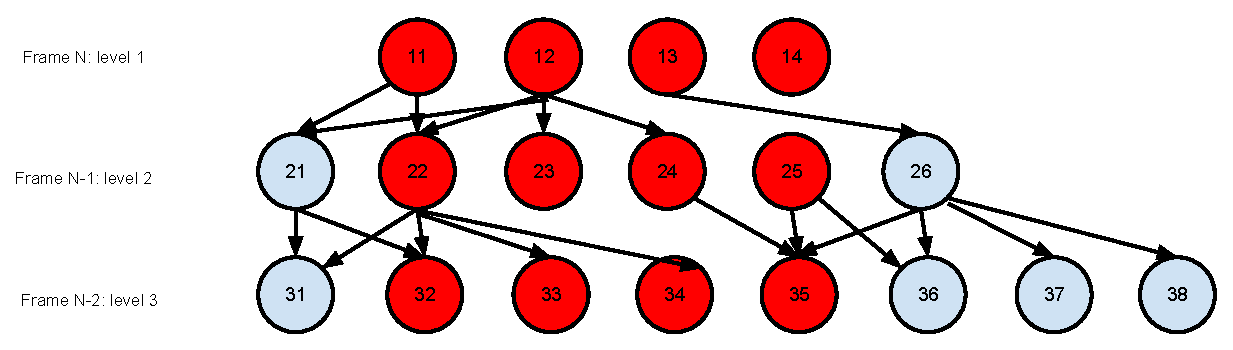
\includegraphics[height=2.5cm]{inter.eps}
\subfigure[Inter-frame Graph]{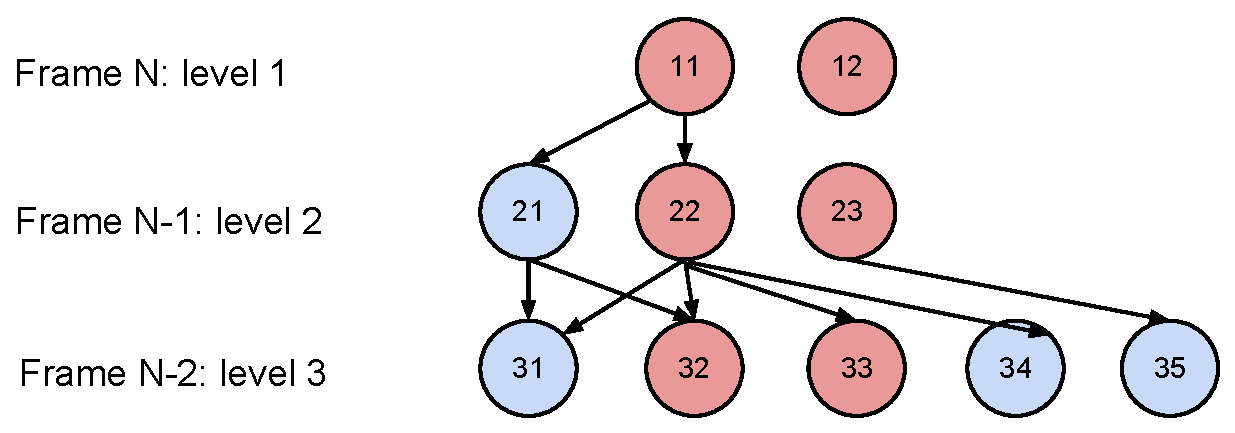
\includegraphics[height=1.6cm]{interc1.eps}}
\quad\quad
\subfigure[Modified Inter-frame Graph]{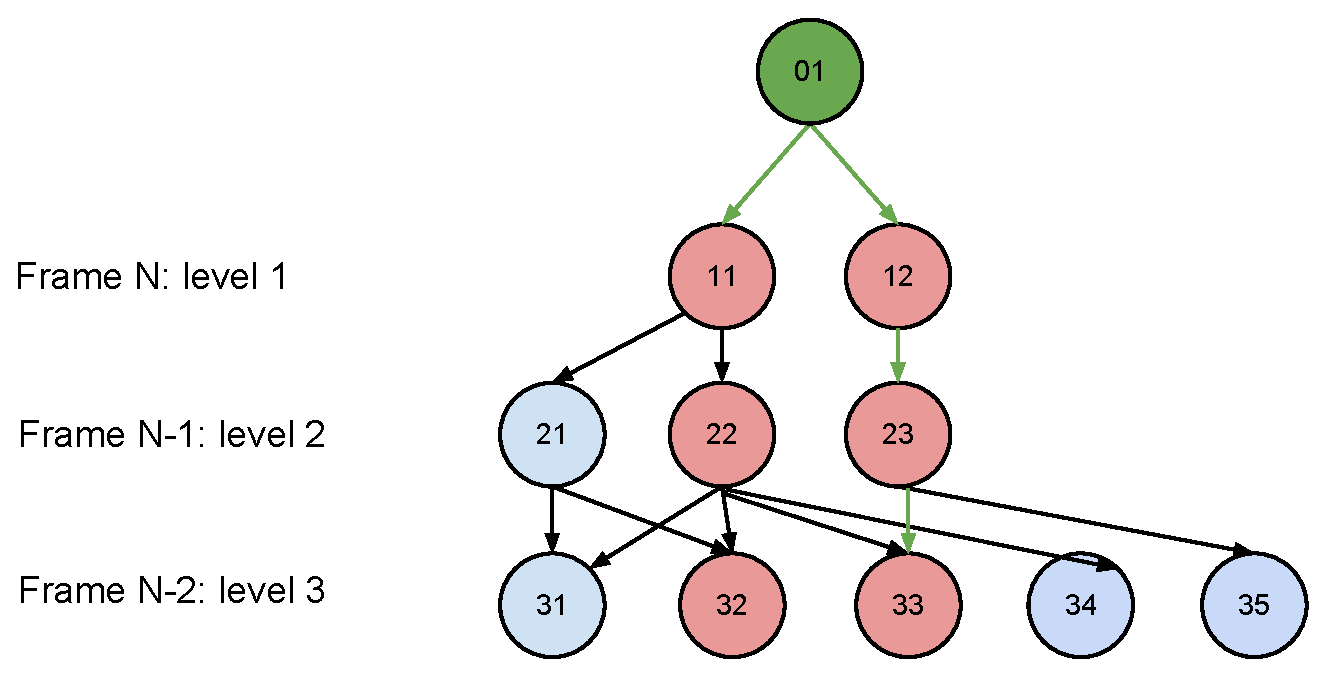
\includegraphics[height=2.5cm]{interc2.eps}}
\caption{Inter-frame Dependency Abstraction} 
\end{figure}
Suppose frame N is the last frame of the GOP, the figure shows the dependencies in three frames. The macroblocks and the dependencies form a graph. By adding a pseudo root node and edges connecting the ROI macroblocks, the graph is transformed to a weakly connected directed acyclic graph shown as Fig 5(b). With this modification, the graph traversal algorithm Depth-First Traversal (DFT) or Breadth-First Traversal (BFT) can be applied. The macroblocks that are visited by the graph traversal are selected, while the rest are not needed. 

\subsubsection{Intra-frame Dependency Computation} 
Similar to Inter-frame dependency, Intra-frame dependency computation can be abstracted to graph traversal problems. 

\begin{figure}
%\vspace{2.5cm}
\centering
\subfigure[Graph]{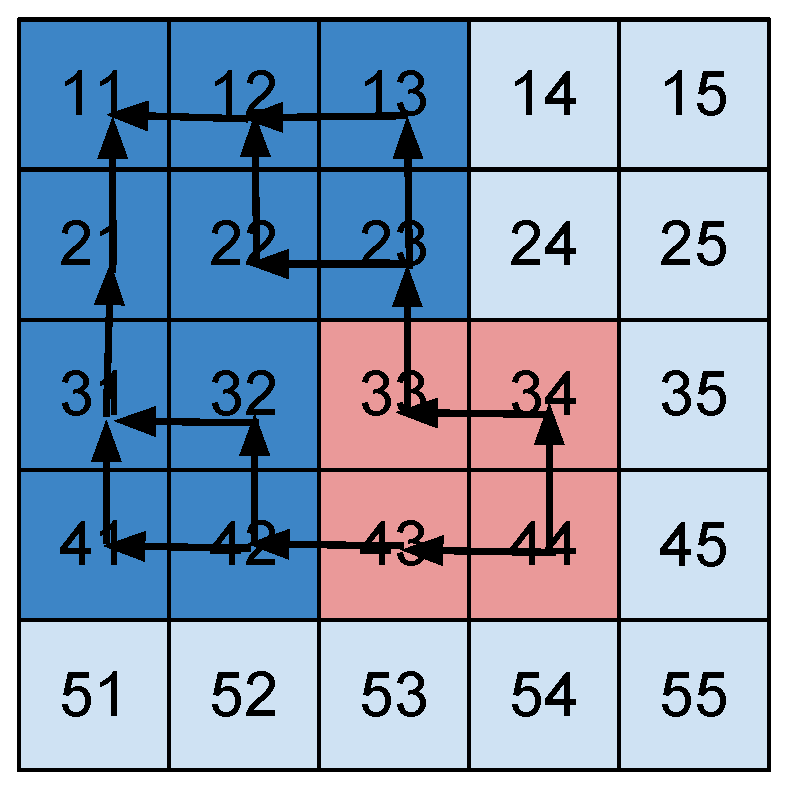
\includegraphics[height=2.2cm]{intrac3.eps}}
\quad\quad\quad
\subfigure[Optimization]{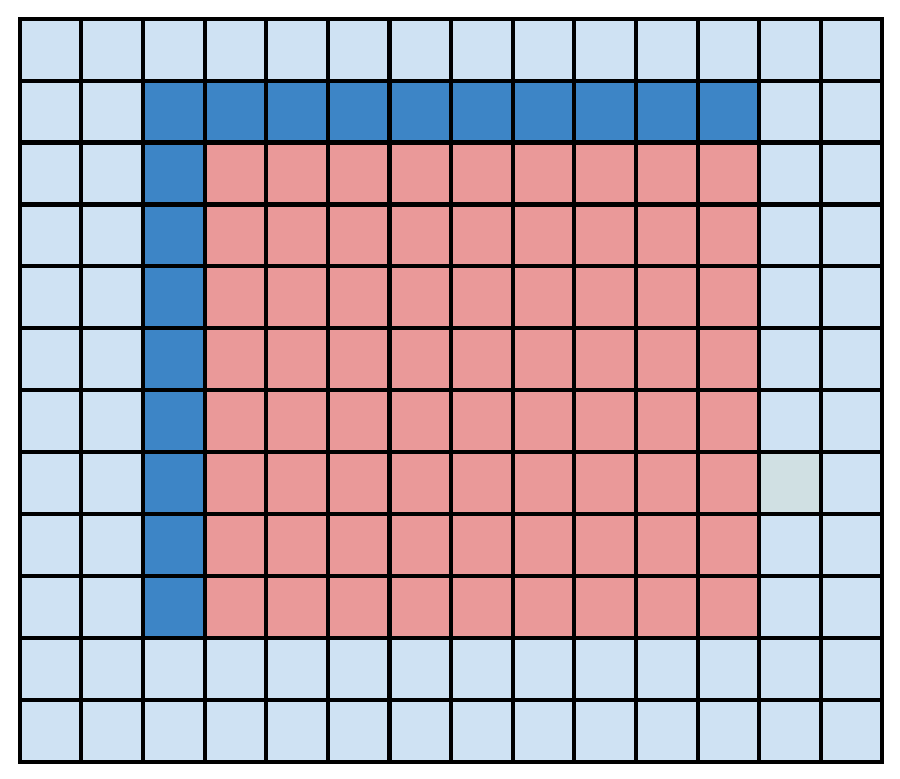
\includegraphics[height=2.2cm]{intrac2.eps}}
%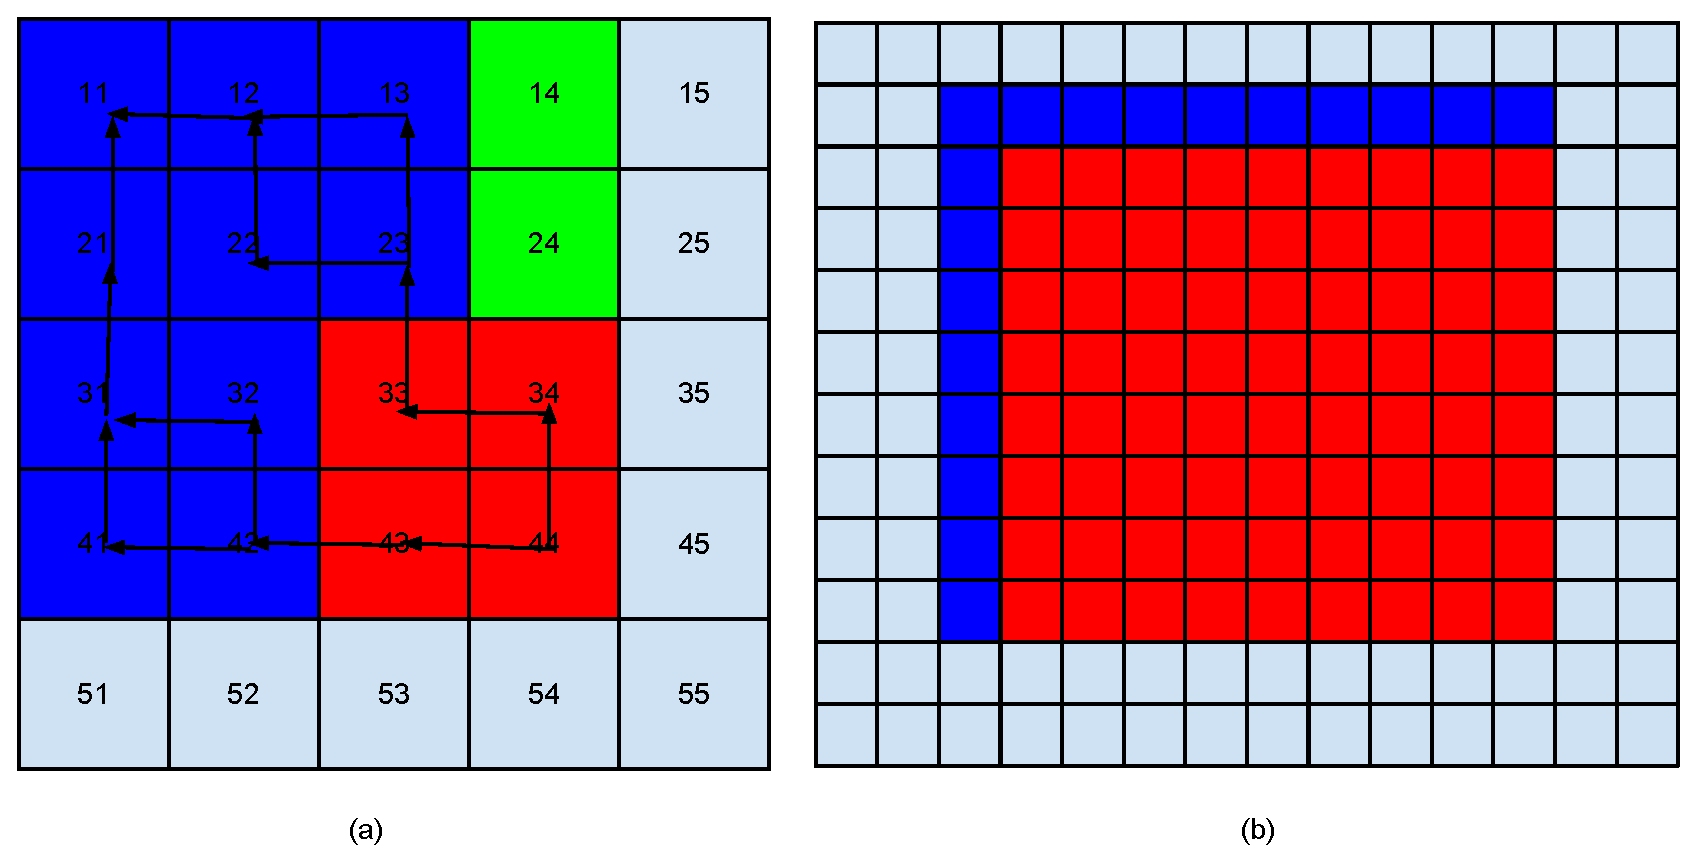
\includegraphics[height=2.5cm]{intra.eps}
\caption[intra.eps]{Intra-frame Dependency and the Optimization}
\end{figure}
In Fig 7(a), macroblock 33, 34, 43 and 44 are ROI macroblocks. The dependency graph due to DC\&AC prediction coding is depicted. Because the dependency direction is always pointing up or left, the graph rooted at a macroblock is always formed by one of the graphs rooted at the first row and first column macroblocks of the ROI and some macroblocks within the ROI. Therefore, an optimization is to apply graph traversal algorithms only on the macroblocks at upper and left edges of the ROI, and select all macroblocks within ROI. This is illustrated as Fig 7(b).

\subsection{Select the Bits}
In order to decode selectively, a mechanism is needed for the decoder to select the bits for selected macroblocks. Two approaches can be used to select the bits, namely bitstream reconstruction and bit seeking. In bitstream reconstruction, a new video bitstream is constructed according to the selective masks and the macroblock start and end positions. The newly constructed bitstream consists of only the macroblocks selected in selective masks. At bit seeking approach, we instruct the decoder to seek to the start position of next selected macroblock at decoding. The second approach avoids the additional memory allocation for the new bitstream therefore it is the preferred approach in our research. However, for applications in the next streaming context, the first approach may provide better bandwidth utilization as the shorter reconstructed bitstream can be transmitted. 

%\subsection{Modifications of Decoder}
%The online computation requires modification for both motion decoding and texture decoding of standard MPEG4 SP decoder. For motion decoding, the MV values are loaded directly from MV dependency file. No MV prediction decoding is carried out. For texture decoding, the DC\&AC prediction direction is read from DC\&AC prediction direction file. mechanism of bits seeking is also added for the decoder to decode selectively. 
  


%\section{Decoding Verification}
Selective decoding is a complicated process with lots of details despite its simple idea and principles. It is important to validate the selective decoding is done correctly. Several approaches can be used. 

The naive approach is simply watch the selective decoded video to see if there is any visible blemishes. A better approach is to compare the selectively decoded ROI pixel values with the pixels decoded by standard MPEG4 SP decoder. A third approach is to compare the output values of each stage of the selective decoding each the values produced by standard decoding. This approach does not only verify if selective decoding is done correctly, but also facilites finding the phase that causes problems if there is any. 




\section{Implementation}
We implemented the techniques and processes described in previous sections on Android platform\cite{webandroid} as a zoomable video player. The architecture of the player is depicted as figure below.
\begin{figure}
\centering
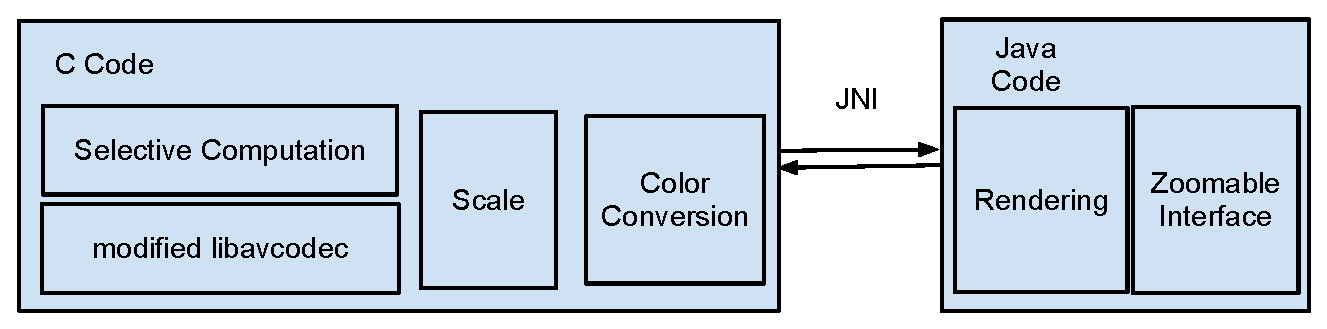
\includegraphics[height=2.5cm]{player.eps}
\caption{Zoomable Video Player Implementation}
\end{figure}
Based on the open source MPEG4 SP codec from libavcodec of ffmpeg 0.7\cite{webffmpeg}, we added the selective decoding functions. At the time of implementation, the ffmpeg codec is not optimized to run on Android platform, especially the scale and color conversion process. We adopts the code from another two open source projects, with scale from libyuv\cite{weblibyuv} and color conversion from Google Chromimum project\cite{webchromium}. 

We implemented the rendering and zoomable interface in Java with Android SDK. The gesture dectector detects a user's pinch or pan gesture, and translates the gesture detected as zoom scale and pan scale. We then compute a ROI from these scales based on what user can see on the phone screen. 

\section{Evaluation}
The purpose of selective decoding is to achieve more efficient zoomable video playback. We evaluate the efficiency of selective decoding from two aspects, video playback frame rate and energy consumption. 

We used a Samsung Galaxy S2 phone for experiment. The device has a dual core processor of 1200 MHz clock rate each and 1024 MB RAM, with Android 2.3.6 running. Two videos of 1080p are used for evaluation, one having little motion while the other containing constant object motion. We refer them as video A and video B respectively. 

\subsection{Frame Rate}
Selective video playback frame rate is affected by both ROI size and position. We designed experiments to examine the influence of each. 

\subsubsection{Different ROI Positions}
Different regions of a video frame may contain different amount of motions and dependencies, therefore the ROI position can affect the amount of processing at decoding and subsequently the video playback frame rate. We fix the ROI size, and then move the ROI from the upper left corner to the lower right of the video frame. The tests are repeated for three different ROI sizes, with the ROI width and height set as 50\%, 70\%, and 90\% of the original video's width and height. 

\begin{figure}
\centering
%\subfigure[Phone A Video 1]{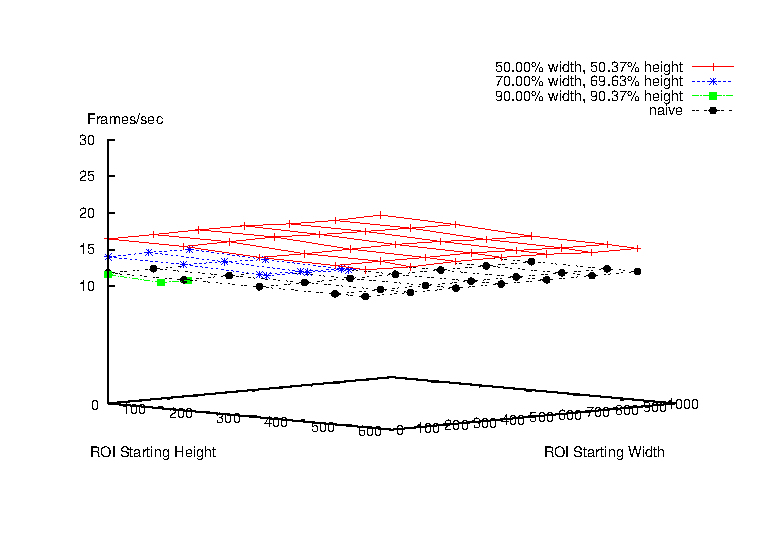
\includegraphics[height=4.0cm]{fr1a1.eps}}
%\subfigure[Phone A Video 2]{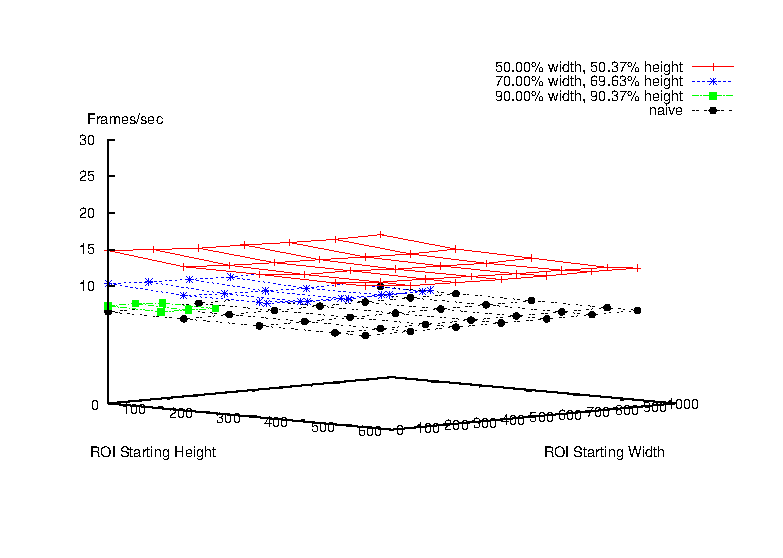
\includegraphics[height=4.0cm]{fr1a2.eps}}
%\
\subfigure[Video A]{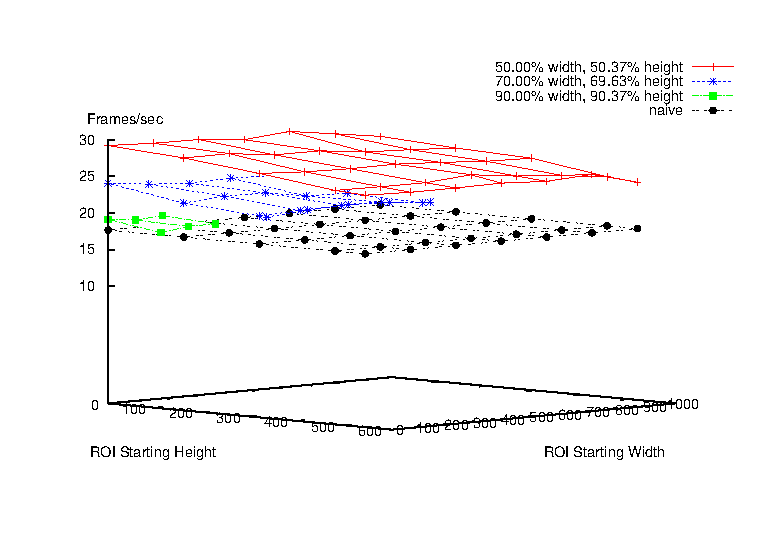
\includegraphics[height=4.0cm]{fr1b1.eps}}
\subfigure[Video B]{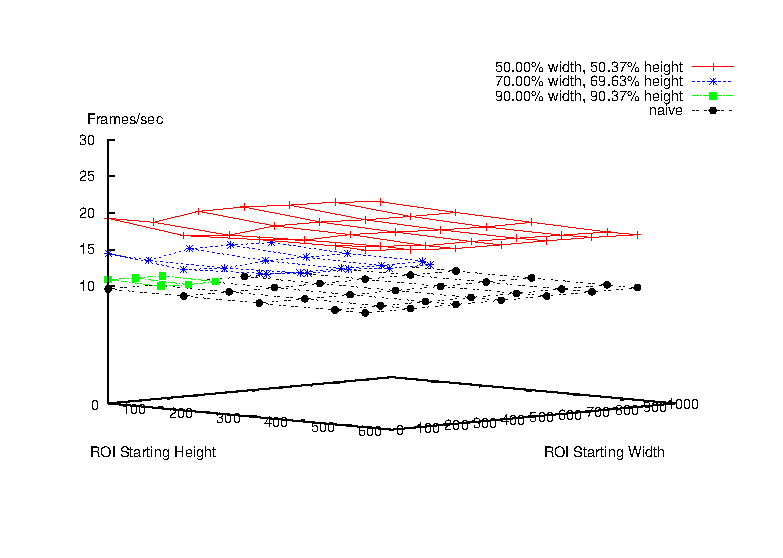
\includegraphics[height=4.0cm]{fr1b2.eps}}
\caption{Frame Rate with 90\%, 70\%, and 50\% of ROI at Different Positions}
\end{figure}
In Fig 8, each 3D interface indicates the frame rate for a ROI size. The intersection in a surface indicates the start position of a particular ROI size. 

Looking at each 3D interface, the frame rate tends to decrease when ROI starting width and/or starting height increases. This is because the intra-frame dependencies increase towards the lower right, and more dependencies cause more macroblocks to be selected and decoded. However, there are exceptions to this decrease trend, which are probably caused by different amount of motions at different ROI positions. Compare different 3D interfaces at a single figure, it is clear that the ROI size has a more significant effect than ROI position and selective decoding outperforms standard decoding. Compare Fig 8(a) with (b), the frame rate for video A is higher than video B. This is expected because video A has less amount of motion than video B. 

\subsubsection{Different ROI Size}
Previous experiment already reveals that ROI size has significant influence on video playback frame rate. This experiment examines the affection of ROI size further. We position the ROI at the center of the video frame and vary the ROI height and width from 10\% to 100\% of original video height and width.

\begin{figure}
\centering
%\subfigure[Phone A Video 1]{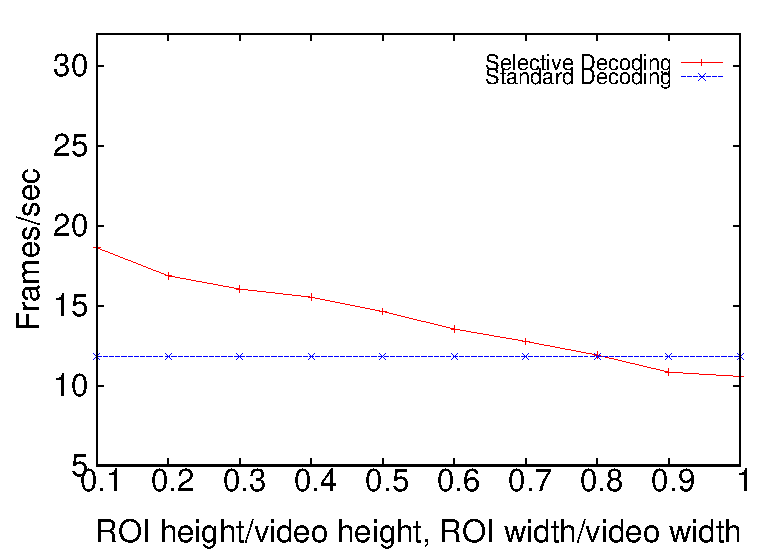
\includegraphics[height=2.0cm]{fr2a1.eps}}
%\subfigure[Phone A Video 2]{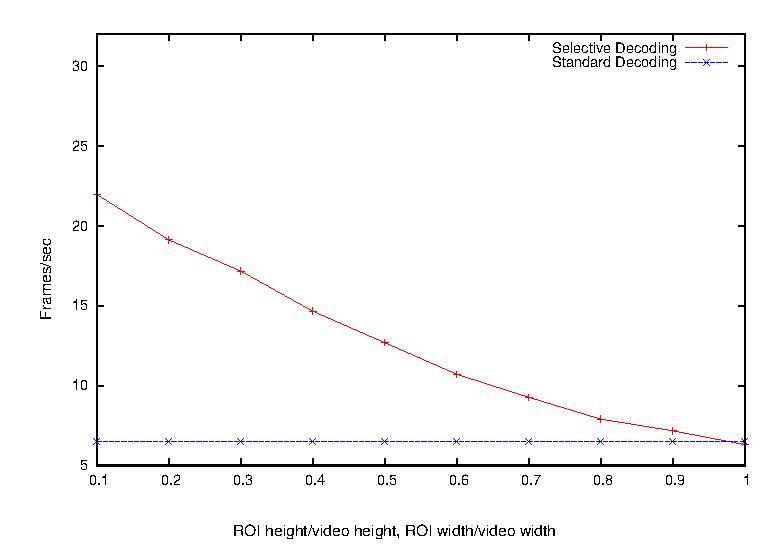
\includegraphics[height=2.0cm]{fr2a2.eps}}
\subfigure[Video A]{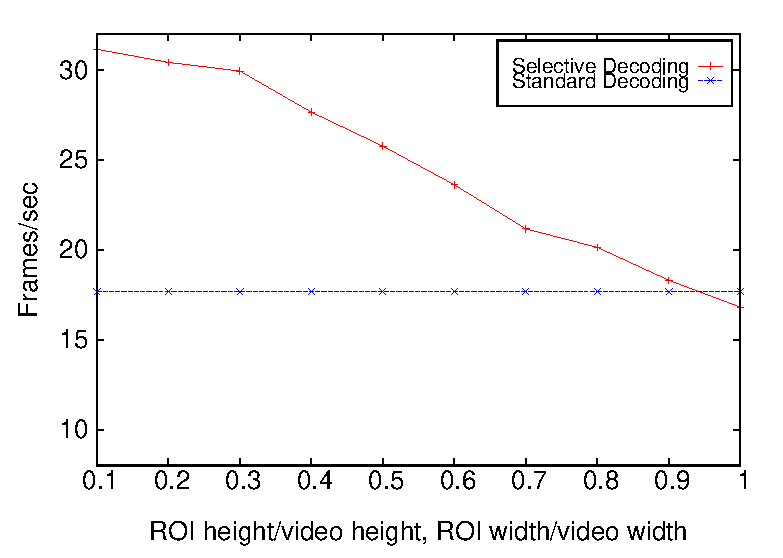
\includegraphics[height=3.0cm]{fr2b1.eps}}
\subfigure[Video B]{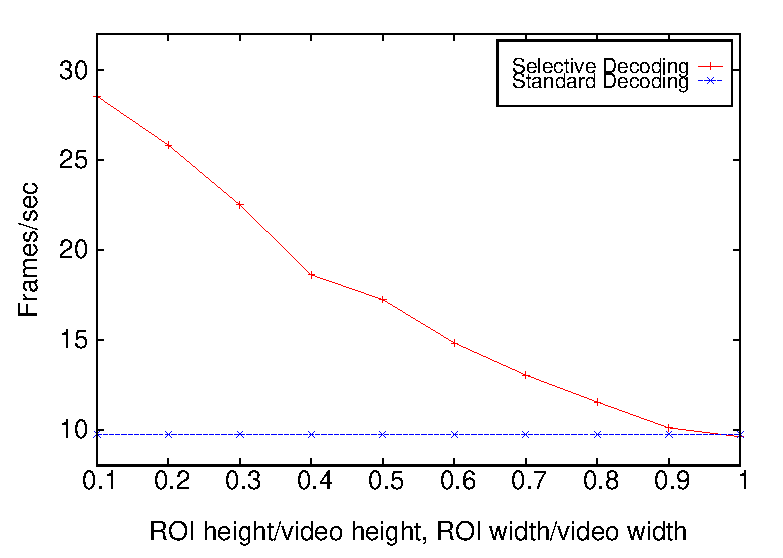
\includegraphics[height=3.0cm]{fr2b2.eps}}
\caption{Frame Rate with 10\% to 100\% ROI Centered}
\end{figure} 
Looking at either Fig 9(a) or (b), frame rate decreases as ROI size increases. Selective decoding achieves higher frame rate at ROI size smaller than 90\%. At 10\% ROI, the frame rate is improved by 76.3\% and 193.3\% for video A and B respectively. The curves at different figures differ due to different amount of motion at center of the video frame. 

%In addition to the two experiments above, we measured the overhead of selective decoding by setting the ROI as the entire frame. The overhead are 4.87\% and 1.34\% for video A and B respectively. In practice, we can switch between selective decoding and standard decoding dynamically based on ROI sizes to achieve higher frame rate. 
 
\subsection{Energy Consumption} 
Energy consumption is the other important aspect of our evaluation. Two experiments are done with different focuses.

\subsubsection{PowerTutor Measurements}
Battery energy is mainly consumed by display and CPU at video playback. PowerTutor\cite{Zhang:2010:AOP:1878961.1878982}, an Android power measurement tool, is capable of measuring power consumed by different hardware components for a user specified app. In this experiment, we vary ROI size from 10\% to 100\%. The frame rate is controlled so that both selective decoding and standard decoding always play at same rate. This is essential for a fair comparison because the CPU display power is dependent on display time. 

For display measurements, we found selective decoding and standard decoding consume almost same amount of energy. However, this is not the case for CPU power consumption, which is shown as Fig 10.
 
\begin{figure}
\centering
%\subfigure[Phone A Video 1]{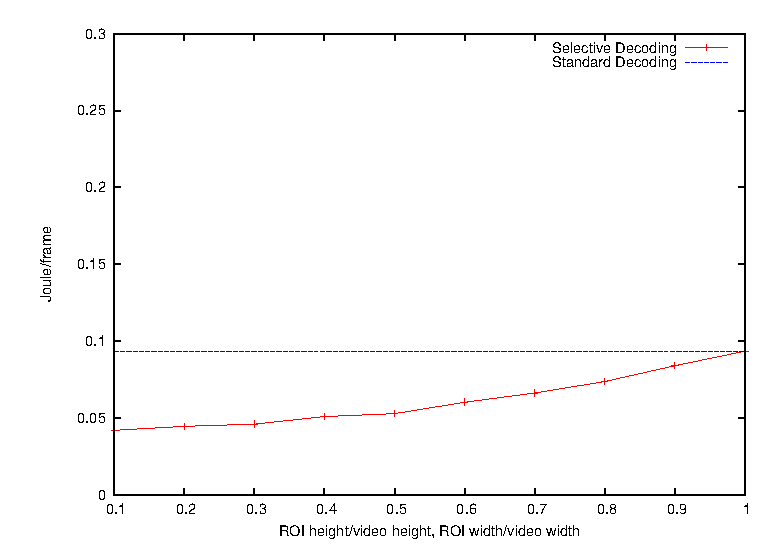
\includegraphics[height=2.0cm]{pta1.eps}}
%\subfigure[Phone A Video 2]{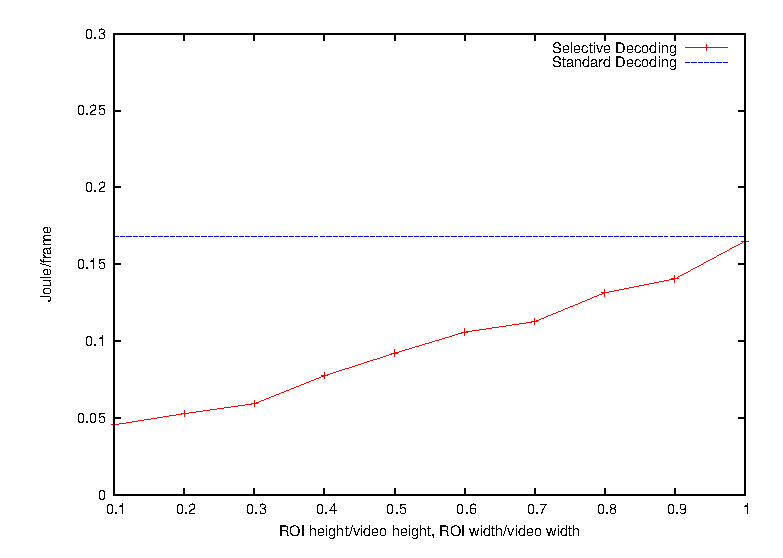
\includegraphics[height=2.0cm]{pta2.eps}}
\subfigure[Video A]{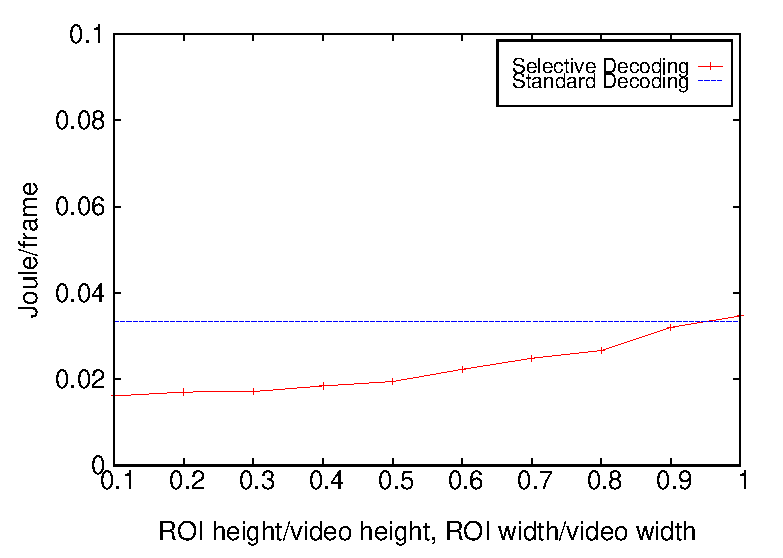
\includegraphics[height=3.0cm]{ptb1.eps}}
\subfigure[Video B]{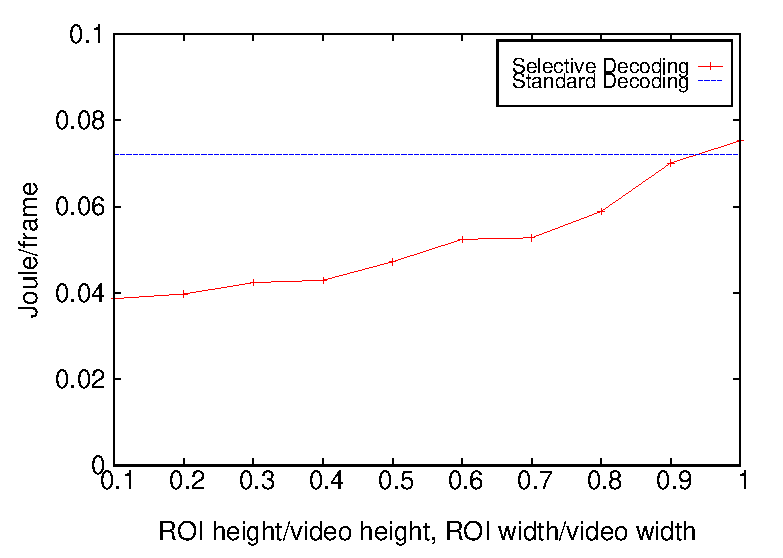
\includegraphics[height=3.0cm]{ptb2.eps}}
\caption{CPU Power Consumption Per Frame}
\end{figure}
Looking at each figure individually, CPU power consumption per frame at selective decoding increases when ROI size increases. At ROI size 90\% or less, selective decoding consumes less CPU energy than standard decoding. Compare Fig 10(a) with (b), video playback for heavy motion video tends to consume more power because of more motion compensation decoding. 

\subsubsection{Power Drain Experiment}
PowerTutor measurements show selective decoding can save energy, mainly by reducing CPU power consumption. However, PowerTutor measurement is obtained through offline-training models\cite{Zhang:2010:AOP:1878961.1878982} and may not be accurate for all phones. We designed another experiment to measure the power consumption. 

\begin{figure}
\centering
%\subfigure[Phone A Video 1]{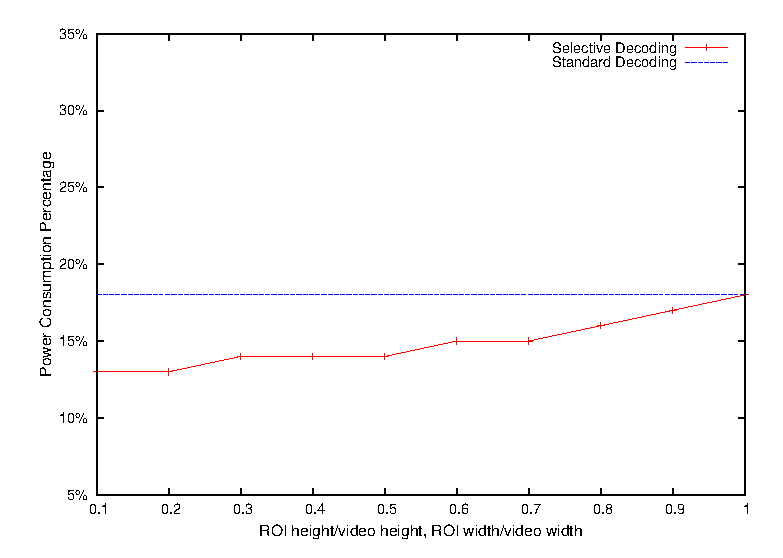
\includegraphics[height=2.0cm]{pwa1.eps}}
%\subfigure[Phone A Video 2]{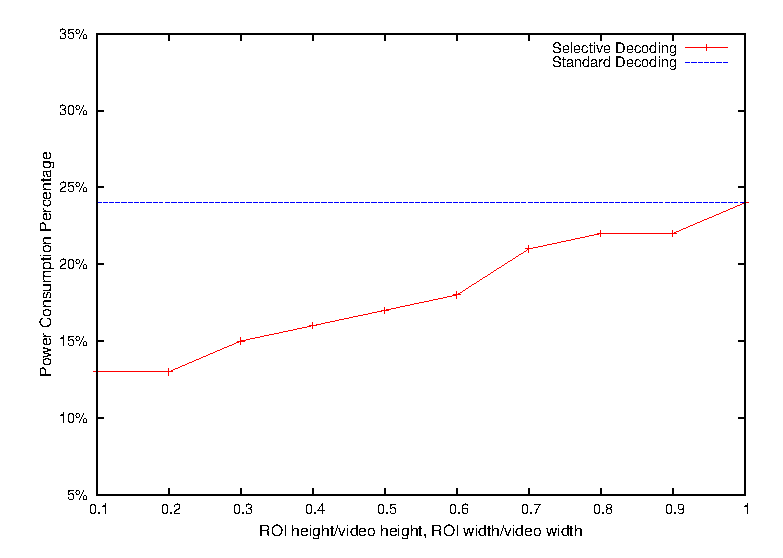
\includegraphics[height=2.0cm]{pwa2.eps}}
\subfigure[Video A]{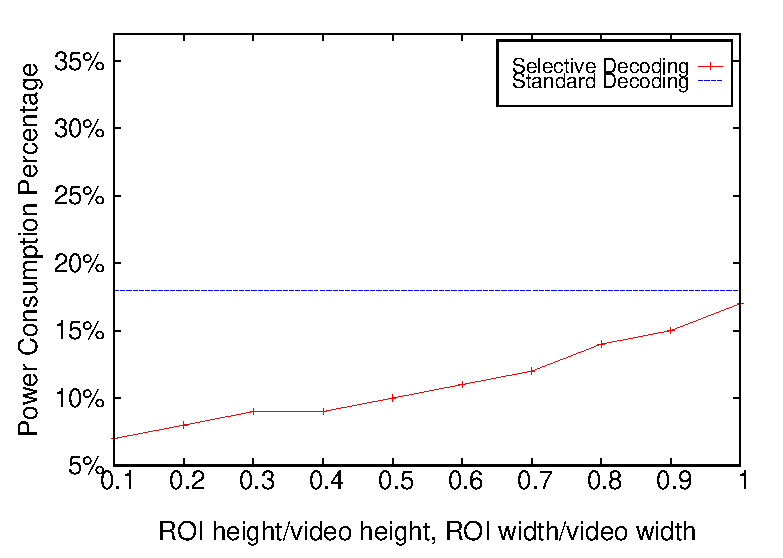
\includegraphics[height=3.0cm]{pwb1.eps}}
\subfigure[Video B]{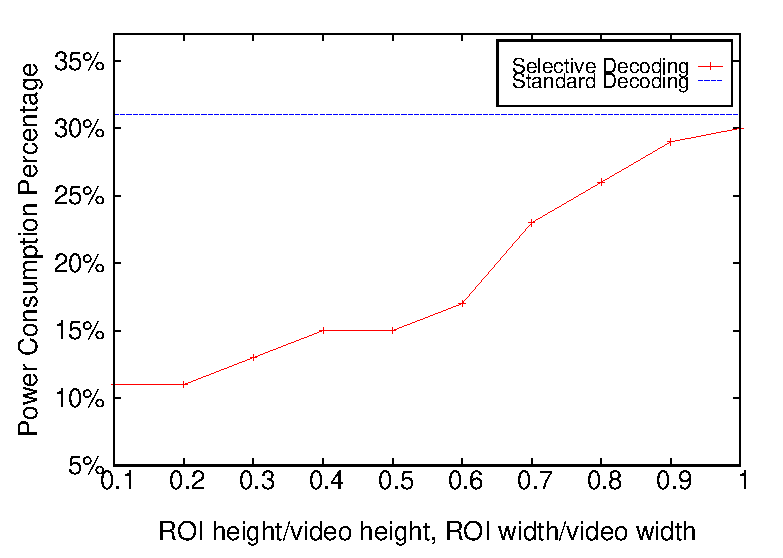
\includegraphics[height=3.0cm]{pwb2.eps}}
\caption{Percentage of Power Drained}
\end{figure}
In this experiment, we place ROI at the video frame center and play the video repeatedly with constant frame rate. Based on the processing power and video, we set the frame rate for two videos as 15 FPS and 8FPS respectively. The percentage of power drained is recorded for comparison. Before each test, we fully charge the phone battery to 100\% and disable all background activities including Wi-Fi, Bluetooth, GPS, etc.

Looking at each figure individually, selective decoding consumes less power. At 10\% ROI size, the battery consumption is reduced by 61.1\% and 64.5\%. Because we set the frame rate differently for videos, the comparison for different videos is not fair and therefore avoided.  

In summary, selective decoding proves to be efficient in terms of playback frame rate and battery energy consumption when ROI size is below certain threshold.  





%\section{Future Work}
Selective decoding presented in this paper illustrates the idea of achieving more efficient zoomable video playback by tracing the dependencies among macroblocks. There are many possible future work can be done based on this simple idea. 
\subsection{Minimize Storage} 
The offline computation of selective decoding prodcues dependency files. The dependency files are plain values stored in binary format. To facilitate memory mapped I/O, heavy padding is introduced to make the records aligned. The table below shows the storage overhead for the two test video sequences.
\begin{table}
\caption{Video Sizes and Dependency File Sizes}
\centering
\begin{tabular}{|c|c|c|}
\hline
Test Video Sequences & Video File Sizes & Dependency File Sizes \\
\hline
Video 1 & 69.0MB & 385.9MB \\
\hline
Video 2 & 88.3 MB & 88.4 MB \\
\hline 
\end{tabular}
\end{table}
One simple idea to reduce storage overhead is to find the limits for stored values and allocate exact number of bits for storing those values. A more complicated but worth exploring approach is to find a better storage scheme to avoid the heavy padding but still be able to access the file quickly in a random fashion. Furthermore, compression can be applied to dependency files. Variable length codes and prediction codes can be used to encode the values. This introduces new computation overhead because the values are compressed at offline computation and de-compressed at online computation. However, it is possible this approach can save a fair amount of space. 

Finally, if we expand the work to encoder and use encoder to generate dependency files, the video file size can be reduced since the duplicated information on dependency files are not needed in video files any more. 

\subsection{Optimize Dependency File Generation}
Our work focuses on optimizing the online computation of selective decoding. The offline computation is carried out once and dependency files are saved. However, the ideal approach is to generate dependency files on the fly when the user is playing the video for the first time. We have worked on a prototype of this approach and it proves working. Because this process is not optimized, we exclude it from our evaluation. 

In addition, as mentioned above, we can generate the dependency files when encoding the video to remove the dependency file generation overhead completely from decoder side. 

\subsection{Encoder Assisted Selective Decoding}
Besides the advantages described above, expanding selective decoding to encoder can bring other research opportunities. The encoding parameters can be adjusted to control the amount of dependenices among macroblocks. However, this could also affect the compression efficiency. Can we configure the encoding parameters to produce videos that achieve an optimal balance bewtween compression efficiency and dependency reduction? 

\subsection{Selective Decoding in Network Streaming Context}
Our work focuses on selective decoding in local playback context. However, it is possible to apply selective decoding in network streaming context. The server side could generate dependency files, compute the seletive masks based on ROI sent from client side, and reconstruct the video bitstream for the client side. Note that this differs from Khiem's \cite{Ngo:2011:AEZ:1943552.1943581} in the way that both encoder and decoder are controlled to work corporately. It is possible that this approach can achieve better bandwidth efficiency than Khiem's work because the decoder can skip the MBs accordingly to the selective masks while Khiem's work assumes a standard decoder.  



\section{Conclusion}
HD video playback on mobile devices needs to be improved. Battery power expenditure is fast at HD video playback and many low end devices suffer from low frame rate.

Based on the fact that users are only interested in part of a video scene at some cases, we designed a software approach named selective decoding to reduce the battery power consumption and increase the frame rate for HD video playback on mobile devices.

Selective decoding is based on analyzing and  tracing various intra- and inter-frame dependency relationships among macroblocks. By doing so, we compute a selective mask which indicates the macroblocks needed to present a clear scene in a user requested ROI. The selective mask  instructs a modified decoder to decode the macroblocks  selectively. The ROI can be captured using a multi-touch gesture interface, which is common in today‟s mobile devices. 


%
% ---- Bibliography ----
%
\bibliographystyle{splncs}

\bibliography{reference}
\end{document}
